\documentclass[conference,10pt]{IEEEtran}
\usepackage{flushend}
\usepackage{lastpage}
\usepackage[utf8]{inputenc}
\usepackage{mathptmx}
\usepackage[dvipsnames]{xcolor}
\usepackage[T1]{fontenc}
\usepackage[english]{babel}
\usepackage{array}
\usepackage{url}
\usepackage{hyperref}
\usepackage{microtype}
\usepackage{graphicx}
\usepackage[binary-units,per-mode=symbol]{siunitx}
\usepackage{cite}

\usepackage{lipsum}
\usepackage{graphicx}

\ifCLASSOPTIONcompsoc
  \usepackage[caption=false, font=normalsize, labelfont=sf, textfont=sf]{subfig}
\else
  \usepackage[caption=false, font=footnotesize]{subfig}
\fi

\def\UrlBreaks{\do\/\do-}

\hypersetup{
  colorlinks=true,% Color URLs with urlcolor
  linkcolor=black,% The color for internal (cross-reference) links
  urlcolor=blue,% The color for URLs (hyperlinks)
  citecolor=black,
  pdftitle={Social Distancing and the Internet: What Can Network Performance Measurements Tell Us?}
}

\urlstyle{same}

% TODO
% - http://www.oecd.org/coronavirus/policy-responses/keeping-the-internet-up-and-running-in-times-of-crisis-4017c4c9/


\begin{document}
\title{Social Distancing and the Internet: What Can Network Performance Measurements Tell Us?}

\author{
    \IEEEauthorblockN{
        \href{mailto:jdm2240@barnard.edu}{\color{black}Jessica Moreira}\IEEEauthorrefmark{1},
        \href{mailto:amey.pasarkar@columbia.edu}{\color{black}Amey Praveen Pasarkar}\IEEEauthorrefmark{2},
        \href{mailto:wc2741@columbia.edu}{\color{black}Wenjun Chen}\IEEEauthorrefmark{2},
        \href{mailto:wh2453@columbia.edu}{\color{black}Kerry Hu}\IEEEauthorrefmark{2},
        \href{mailto:janakj@cs.columbia.edu}{\color{black}Jan Janak}\IEEEauthorrefmark{3},
        \href{mailto:hgs@cs.columbia.edu}{\color{black}Henning Schulzrinne}\IEEEauthorrefmark{3}
    }
    \IEEEauthorblockA{
        \IEEEauthorrefmark{1}Barnard College, New York, USA
    }
    \IEEEauthorblockA{
        \IEEEauthorrefmark{2}Fu Foundation School of Engineering and Applied Science, Columbia University, New York, USA
    }
    \IEEEauthorblockA{
        \IEEEauthorrefmark{3}Department of Computer Science, Columbia University, New York, USA
    }
    Email:
    jdm2240@barnard.edu,
    \{%
      \href{mailto:amey.pasarkar@columbia.edu}{\color{black}amey.pasarkar},%
      \href{mailto:wc2741@columbia.edu}{\color{black}wc2741},%
      \href{mailto:wh2453@columbia.edu}{\color{black}wh2453}%
    \}@columbia.edu,
    \{%
      \href{mailto:janakj@cs.columbia.edu}{\color{black}janakj},%
      \href{mailto:hgs@cs.columbia.edu}{\color{black}hgs}%
    \}@cs.columbia.edu
}

\maketitle

\begin{abstract}
The COVID-19 outbreak has changed the way that people interact. With the new stay-at-home and social distancing orders, most activities that people were used to changed drastically, e.g., going to work and classes, living on campuses and traveling. In this new social environment, since early March people in the United States were required to quarantine and do all their activities from home. Thus, in this project we researched how COVID-19 has impacted internet usage in the  United States. While analyzing the fixed broadband raw data sets collected by the Federal Communications Commission (FCC), we were able to identify how aspects of internet usage such as amounts of data downloaded and uploaded by users and the average download and upload speed changed due to COVID-19. Moreover, through this analysis, we could also learn about how people have changed their behaviors while using the internet during COVID-19.
\end{abstract}

\section{Introduction}
\label{sec:introduction}

Much has been written about whether the residential internet infrastructure in the United States can cope with the sudden conversion of work into tele-work, school into distance learning and movies into Netflix binging, albeit usually based on data of dubious quality. But network measurements may also tell us about the effort and success of social distancing, the ability of different communities to move to internet-mediated modes of interaction and their sustainability.

We attempt to address both questions in this paper. First, we describe some of the sampling bias limitations of classical user-initiated network speed measurements in estimating how well infrastructure holds up during shifts in usage. For example, seeming reductions in speed may be caused by increased Wi-Fi interference or simply by increased usage by people who have lower internet speeds, whether by deliberate choice, availability or affordability.

We then draw on the FCC Measuring Broadband America (MBA) raw data, available longitudinally since 2011, to estimate the impact of increased internet usage on a variety of performance metrics, including throughput, latency and packet loss, disaggregating by coarse-grained geography and technology. Even though it usually does not draw much attention, we are particularly interested in upstream performance, as much more intense use of video conferencing tools has been shown to increase upstream bandwidth usage by 10-40\%.

At least as important as measuring the impact of COVID-19 on internet performance is using indirect metrics, such as internet usage, to estimate the success of social distancing measures, while maintaining user privacy. We draw on two metrics to explore whether we can detect the daytime and evening usage of residential internet users, indicating home schooling and work from home, as well as observance of stay-at-home orders on weekends. MBA suspends throughput measurements during periods of significant usage, such as video conferencing, and also tabulates total use. Thus, we might be able to deduce when households are actively using their broadband connection and whether such usage reflects, for example, the earlier restrictions imposed in Washington State or in the New York City metro area.

The measurement data has known limitations. For example, it only covers the largest ISPs and omits fixed wireless and satellite providers, the latter by their choice. We describe how more systematic data gathering during both short-term natural disasters and long-term epidemics could supplement our understanding of how households deal with such crises, providing information to policy makers in near real-time and in a privacy-respecting manner.

% Due to government imposed lockdowns, a large percentage of the population had to depend in residential broadband internet connection for work, entertainment, education, and social activities.

In early March, the US was hit by the COVID-19 outbreak. In order to control the spread of the virus and flatten the infection curve, states throughout the country implemented stay-at-home orders which forced people to quarantine. Thus, as people started quarantining at home, many started executing their daily activities, e.g., having social gatherings from home in an online environment.

Thus, considering this new format of social interaction caused by COVID-19, this study aims to understand how this virus has impacted internet usage in the United States. It identifies the changes in internet usage caused by the COVID-19 outbreak, e.g., change in the average downloaded and uploaded data consumption, in the average download and upload speed, in the peak periods of usage, and in latency. By observing the changes in the way that internet has been used, this study also infers and presents information about people's behavior during COVID-19, e.g., if people complied with stay at home orders, engaged in online learning, and worked from home.

In the following sections of the paper we present related work about the impacts of COVID-19 in internet usage (Section \ref{sec:related-work}), information about the data set (Section \ref{sec:datasets}) and the environment used to process and analyze the data (Section \ref{sec:methodology}) and then the results achieved by analyzing the data (Section \ref{sec:data-analysis}). Moreover, we also present the challenges that we faced while executing this project (Section \ref{sec:challenges}). Finally, we conclude and discuss future work in Section \ref{sec:conclusion}.

\section{Related Work}
\label{sec:related-work}

%\nocite{fcc-pledge}
%\nocite{nanog}
%\nocite{partridge2003internet}

A small number of studies focusing on the effects of lockdowns on internet infrastructure have already been published as of November 2020. These studies typically look at traffic trends and patterns from various vantage points. Some look for signs of stress in internet infrastructure, others attempt to correlate traffic data with user behavior during lockdowns.

Feldmann et al. studied the effects of lockdown on internet traffic using traffic data obtained from several Internet Service Providers (ISPs) and Internet Exchange Points (IXPs) in Europe and the US East Coast\cite{feldmann2020lockdown}. The authors found that residential traffic increased by 15-20\% after the lockdown and that remote work and education applications saw a 200\% increase in traffic. The regular weekday traffic pattern morphed into a weekend-like pattern with a significant traffic increase starting in the morning, from mid-March until roughly mid-May.

B\"{o}ttger et al. studied similar effects using data from Facebook's global edge network \cite{bottger2020internet}. They observed a traffic increase in the second half of March and found regional correlations between traffic growth and the spread of COVID-19 in the region. The data from Facebook's video services showed a degradation in the quality of user experience in India and South Africa. Authors attribute the degradation to limited capacity and last-mile network congestion in those countries.

Liu et al. found a 30-60\% increase in peak traffic volumes in the US, a statistically significant increase of 10\% in average latency over two months, and ISPs adding interconnect capacity at more than twice the usual rate \cite{liu2020characterizing}.

Several broadband market reports analyze the state of broadband infrastructure during the pandemic. OpenVault saw a 40\% broadband traffic increase in 3Q 2020 over 2019, but less than 1\% over 2Q 2020 \cite{openvault}. Traffic growth plateaued in 2020, indicating a new normal for broadband bandwidth usage. Temporarily relaxed data usage quota resulted in faster growth of usage-based accounts compared to flat rate accounts. Ofcom reports that UK broadband service providers were generally able to keep up with the demand in March, with only a 1-2\% decrease in download and upload speeds and 2\% increase in latency \cite{uk-home-broadband-performance}. SamKnows published a series of articles about the state of critical infrastructure \cite{samknows-cdn,samknows-video-streaming,samknows-video-conferencing,samknows-usa}. Their observations in UK and the US show only slightly worse average download speeds and round trip times during lockdown.

Several network service providers discuss lockdown-related trends and observations on their blogs: Google \cite{google}, Akamai \cite{akamai}, Facebook \cite{facebook}, Comcast \cite{comcast}. In all cases, initial traffic surges aligned with mandatory isolation protocols have been reported, as well as long-term shifts in diurnal and weekly traffic patterns. The general sentiment appears to be that existing infrastructure was either able to keep up with the traffic due to over-provisioning, or could be rapidly adapted to meet the increased demand. It is worth mentioning that network service providers generally report higher traffic surges than broadband monitoring companies like SamKnows or OpenVault.

NCTA reports a usage growth of 30\% (downstream) and 50\% (upstream) since March among its member broadband cable providers \cite{ncta}. Sandvine saw a traffic growth of 40\% between February and April. The growth was driven by video, gaming, and social sharing applications which comprise 80\% of all traffic \cite{sandvine}.

Kovacs compared the performance of fixed broadband internet during the pandemic in the US and in Europe \cite{kovacs}. Using data collected by the company Ookla, the author found that US fixed broadband networks generally performed better than their comparable European peers, offering 30-35\% higher mean download speed. Kovacs attributes the difference to bigger long term investments in telecommunications infrastructure, more favorable mix of technologies, and lighter-touch regulatory approach in the US.

% Another article \textit{Stealth CEO: Asymmetric broadband speeds cause strain during work from home efforts} \cite{robuck} points out that people who are currently working from home have faced some challenges to open all their work applications and have been using more cloud services. According to Robuck, internet traffic caused by these cloud services increased 32\% since staying-home orders started in the country. Moreover, it has been confirmed that people have experienced an asymmetrical connection which has directly slowed the upstream speed.

% Moreover, according to Frankel \cite{frankel}, the average down streams in urban spaces in March 16th was \SI{5.1}{\giga\byte} - more than double of the down streams value registered nine weeks before. In addition to that, Frankel affirms that according to Nilsen, video streaming consumption increased 61\% in the US since early March.

Lutu et al. studied traffic patterns obtained from a UK-based mobile network operator (MNO) and analyzed the effect of mandatory stay-at-home orders on users' mobility behavior \cite{lutu2020mobile}. They found an overall decrease in users' mobility following the government’s mandatory stay-at-home orders. The authors found a decrease in cellular data traffic volumes and an overall increase in voice traffic.

\section{Datasets}
\label{sec:datasets}

The Federal Communications Commission (FCC) runs a program called Measuring Broadband America (MBA) which collects data about broadband internet usage and performance in the United States \cite{mba}. The data is collected by a panel of volunteers with a hardware monitoring device installed on their fixed broadband internet connection. The device is known as the whitebox and is manufactured by SamKnows \cite{sam}. The panel consists of 4000 to 5000 volunteers (depending on the year), selected by the FCC to include 16 major ISPs, geographic regions, and broadband connection types \cite{fcc-report-appendix}. The whitebox uses a combination of passive and active measurement techniques to determine the state, parameters, and usage of the internet connection repeatedly throughout the day.

Since 2011, the FCC has been publishing annual reports on the overall performance of the US fixed broadband infrastructure \cite{mba-studies}. The reports are based on the data collected from a representative subset of the whiteboxes, cross-validated with information provided by broadband ISPs. The reports cover approximately 80\% of the US population.

In addition, the FCC regularly publishes anonymized raw datasets on its website \cite{data}. All deployed whiteboxes generate approximately \SI{20}{\giga\byte} of data per month. In this study, we use the raw datasets to analyze the performance and changing usage patterns of US fixed broadband before and during COVID-19 related government-imposed restrictions (lockdowns). We work with the raw data collected from January 2019 to June 2020.

The raw datasets are published in the form of comma-separate values (CSV) files broken down by the month and type of measurement. The following measurements are included: upload and download speed, the time to fetch a few selected well-known web pages, UDP/ICMP latency when idle and under load, video streaming performance, VoIP performance, DNS performance, and total bytes uploaded and downloaded by the user. In this project we only use the following raw data subset: upload and download speed, total user bytes, and latency.

In addition to raw data sets, we also use the unit profile, unit census block, and excluded units datasets as published by the FCC. The unit profile dataset provides additional information about whiteboxes, including ISP name and service tier, technology, and coarse location. Not all whiteboxes are included in the unit profile dataset. The unit census block dataset identifies the census block for each whitebox. The excluded units dataset lists the whiteboxes that were excluded from the annual report. At the time of this study, the most recent unit profile, unit census block, and excluded unit datasets were from 2018, i.e., considerably older than the raw data.

Analysis that involves population demographic information integrates 2019 U.S. Census data \cite{census}. We use the population dataset that provides county-level population information.

The size of all the datasets used the analysis presented in this paper was more than \SI{300}{\giga\byte}, requiring the use of big data workflows. By analyzing these data sets, we were aiming to understand not only how internet usage has changed, but also how people's internet usage behavior has changed over the course of the pandemic.

\subsection{Ethical and Privacy Considerations}
\label{sec:ethical-and-privacy-considerations}

The FCC MBA panel consists of volunteers who were informed regarding the details of the program, explicitly opted into the program, and provided written consent to participate. All publicly released FCC MBA datasets have all personally identifiable information removed.

All additional datasets used in this study, e.g., the U.S. Census Bureau data, is public information and can be obtained freely from the internet.

\section{Methodology}
\label{sec:methodology}

In order to analyze the impacts of COVID-19 lockdowns on fixed broadband internet usage, we need to analyze and compare data from time periods before and during lockdown. In the US, the states issued statewide lockdown orders on different dates. Table \ref{tab:state-lockdown} shows the date of the statewide lockdown order for selected states. The first state to issue a lockdown order was California on March 19. The last statewide lockdown order was issued by South Carolina on April 7. Seven states did not impose lockdown orders.

\begin{table}
  \centering
  \caption{Lockdown dates for selected U.S. states}
  \label{tab:state-lockdown}
  \begin{tabular}{ |c|c| }
    \hline
    State         & Lockdown date \\
    \hline
    Arizona       & March 31 \\
    California    & March 19 \\
    Florida       & April 2  \\
    Illinois      & March 21 \\
    Massachusetts & March 24 \\
    New Jersey    & March 21 \\
    New York      & March 20 \\
    Texas         & April 2  \\
    \hline
  \end{tabular}
\end{table}

Thus, for the purpose of the analysis presented in this paper, we use January and February 2020 as the pre-lockdown period. We use the second half of March and April as lockdown period. To eliminate seasonal effects, we also use the data from January-April 2020 for comparison in some of the analysis. Thus, most of our algorithms run on the data from January 2019 to June 2020 (the last dataset published by the FCC as of September 2020).

We uploaded the FCC MBA raw data from January 2019 to June 2020 into Google Cloud BigQuery \cite{bigquery}. We then analyzed the data using Google Cloud Datalab \cite{datalab} running on virtual machines (VMs) in Google Cloud. Google Cloud Datalab is a version of JupyterLab \cite{jupyter} with Google Cloud specific extensions (e.g., libraries to access the BigQuery database). All our scripts to process the data were written in Python 3. We kept everything synchronized and organized in a shared Git repository.

% TODO: talk about how the data is cleaned (outliers, excluded units, unit profile)

\subsection{Population Demographics Analysis}

We are provided with Federal Information Processing Standard (FIPS) codes for users in the study ($n=1692)$. These codes provide information regarding user's county of residence. We determine the population of these counties using open-source 2019 US Census Data. The specific census dataset provided populations for each county in the US and was processed with SQL.

We classify users as belonging to a 'Metro' area if their corresponding county population is greater than $1,000,000$ ($n=396$). Similarly, we classify users as belonging to a 'Rural' area if the county population is less than $100,000$ ($n=342$). To ensure that any trend we observe over time is not due to shifting demographics, we focus specifically on users who have participated in the study since January $2019$.

\subsection{Hourly Usage Patterns}

In this part, we will compare the average downloaded data per user over hour and the average uploaded data per user over hour on each month before and after COVID-19. The downloaded data is the number of bytes that the customer received from the internet to wired LAN devices and the Wi-Fi devices, and the uploaded data is the number of bytes that the customer transmitted from wired LAN devices and Wi-Fi devices to the internet.

Since the recorded time in data set is finished in coordinated universal time, in order to get the time of download or upload event at local time, we add the time zone offset from the user profile to the recorded time.  We extract the year, month, and hour from the local time, and handle some special cases: (1) for hour, there is some location behind coordinated universal time and if the hour in local time is negative, add the value by $24$. (2) For month, if the value of hour in local time is negative and the day is $1$, we subtract the value of extracted month by 1 because it will be the last date of the previous month, and (3) for year, if the value of hour in local time is negative, the month is 1 and the day is 1, we subtract the value of extracted year by 1 since it will be the last date of the previous year. For the users, we focus on users who are present throughout the course of the study. We notice that the number of bytes that the customer transmitted from wired LAN devices to the internet for some users is the value of maximum integer. The possible reason is that the device measuring that value may be broken so we ignore all the users who have those values.

For each month, the average number of downloaded data and that of uploaded data are defined as

\begin{equation}
    AVG_{\text{download}} =\frac{SUM(\text{download data})}{COUNT(\text{persistent users})}
\end{equation}
\begin{equation}
    AVG_{\text{upload}} =\frac{SUM(\text{upload data})}{COUNT(\text{persistent users})}
\end{equation}
where ``persistent users" means the users who are present throughout the course of the study.

\section{Data Analysis}
\label{sec:data-analysis}
\begin{figure*}[t]
    \centering
    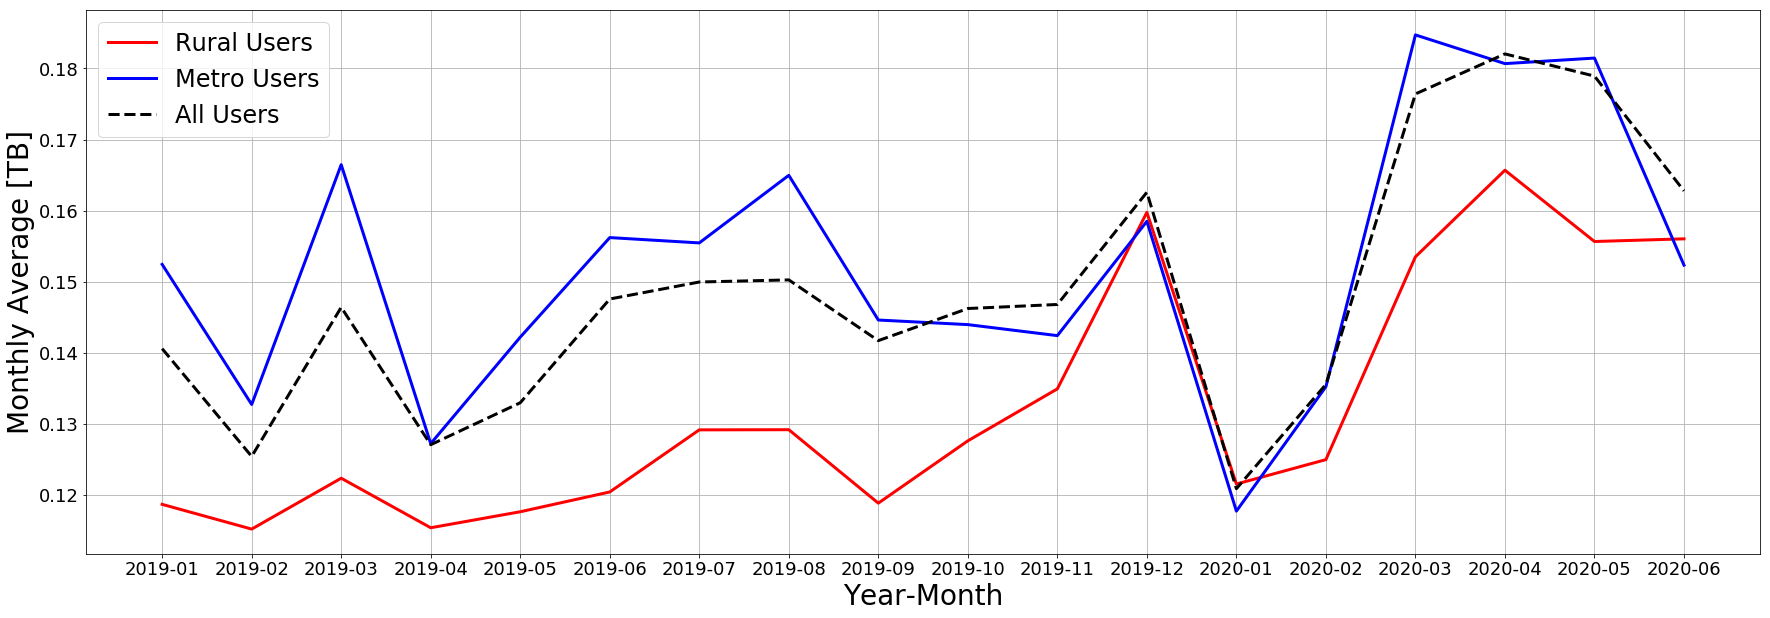
\includegraphics[width=1.0\linewidth]{figs/monthly_downloaded_data_notitle.png}
    \caption{Graph showing the monthly average downloaded data per user from January 2019 to June 2020, partitioned by test unit county population.}
    \label{fig:downloadmetro_rural}
\end{figure*}

\begin{figure*}[t]
    \centering
    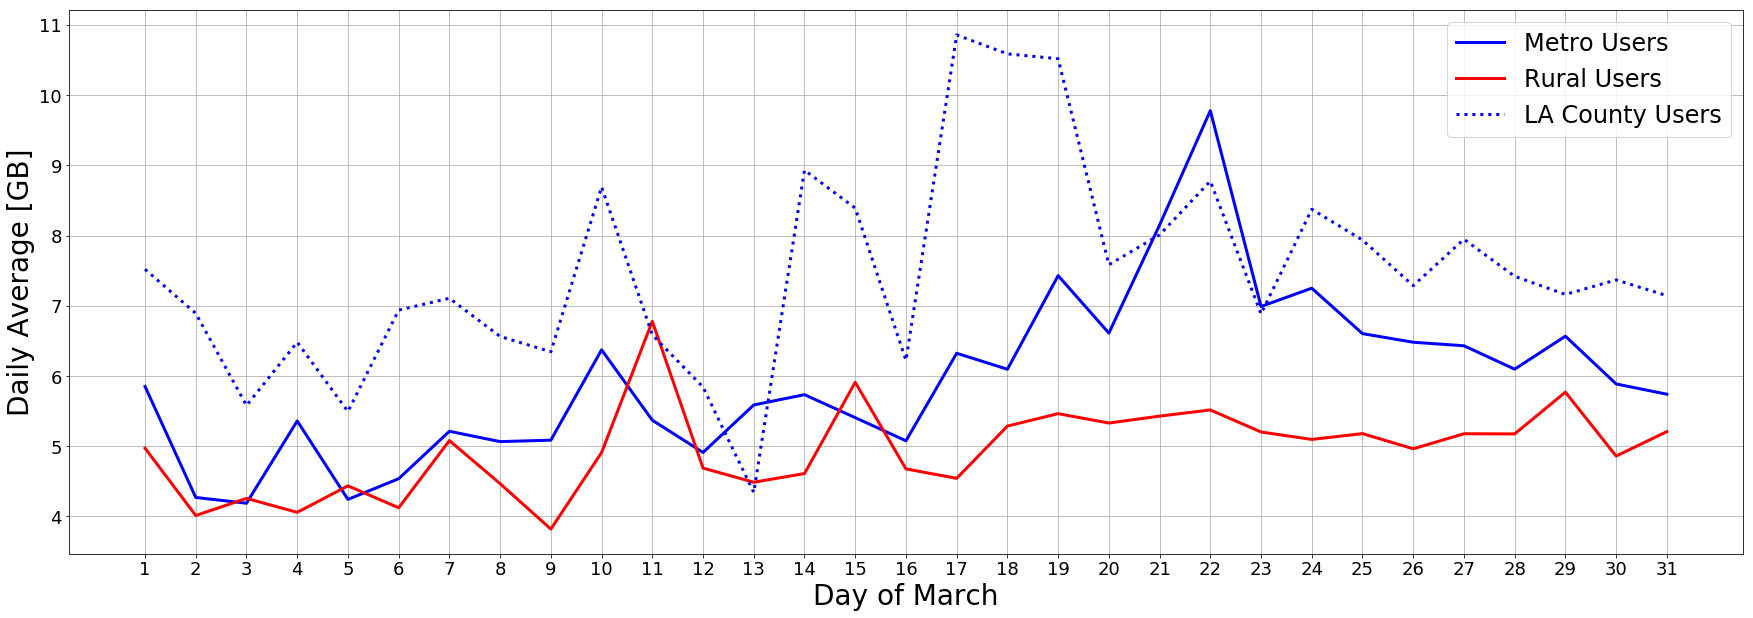
\includegraphics[width=1.0\linewidth]{figs/daily_downloaded_data_notitle.png}
    \caption{Graph showing the daily downloaded data per user in March 2020 for those in metro and rural areas, as well as LA county.}
    \label{fig:dailymetro_rural}
\end{figure*}

\section{Data Usage by Population Demographics}
\label{sec:data-usage-by-population-demographics}

\subsection{Average Monthly Downloads}

A high-level overview of the effect of COVID-19 on fixed broadband internet usage can be seen by analyzing the average monthly downloaded data per user. As can be seen in Figure \ref{fig:downloadmetro_rural}, we notice a sizable increase in overall downloaded data in the months of March, April, and May 2020. This increase is consistent across both metro and rural counties, although it is more pronounced in metro areas. The three pandemic months are the highest-usage months for metro areas. In contrast, rural areas only have one month larger than their pre-pandemic maximum of December 2019. 

Interestingly, in the fourth month of the pandemic, we notice a drop in overall downloaded data in metro areas, while rural areas remain constant. This drop coincides with the relaxation of many stay-at-home orders, indoor dining bans, and curfews in cities across the United States \cite{money2020la,gov2020nyc}. 

% \begin{figure*}
%     \centering
%     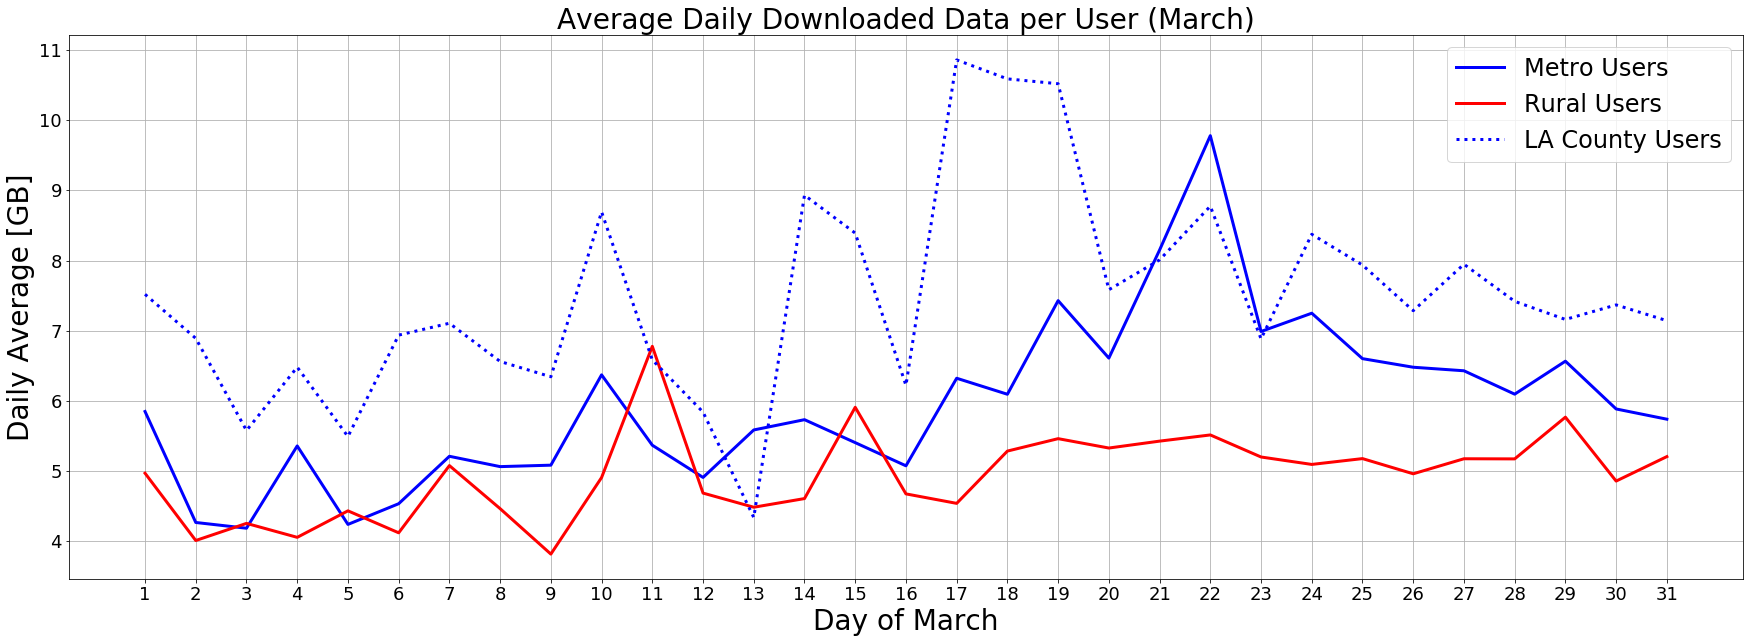
\includegraphics[width=1.0\linewidth]{figs/daily_downloaded_data.png}
%     \caption{Graph showing the daily downloaded data per user in March 2020 for those in metro and rural areas, as well as LA county.}
%     \label{fig:dailymetro_rural}
% \end{figure*}

\subsection{Average Daily Downloads}
Focusing on daily fixed broadband internet usage can allow us to understand the public's reactions to various events. In particular, by analyzing daily overages over the course of March, we can better understand the reactions to the various stay-at-home orders, school shutdowns, and curfews from an internet usage point-of-view. 

To this end, we present in Figure \ref{fig:dailymetro_rural} the daily average downloaded data usage for both metro and rural users. The first event we look to analyze is the White House first announcing its social distancing recommendations on March 16 for the entire country \cite{trump2020coronavirus}. Following this announcement, we observe that users in metro areas use a significantly larger amount of data than those in rural areas. In the first half of the month, there was no such difference (Figure \ref{fig:dailymetro_rural}). It is unsurprising that those in cities and other metro areas reacted to this recommendation more drastically than those in less populated areas. Cities such as New York City, San Francisco, and Los Angeles (LA) were among the hardest hit areas in the early weeks of the pandemic \cite{cdc2020tracker}. 

For many of the aforementioned cities, various levels of lockdowns were put in place on top of the White House's recommendations \ref{tab:state-lockdown}. Therefore, we additionally investigate if we can correlate these local ordinances with county-level usage patterns. Los Angeles (LA) county has the most test units in the FCC MBA dataset ($n=44$), so we examine the daily average downloaded data per user for all those residing in LA (Figure \ref{fig:dailymetro_rural}). 

We observe the first large spike on March 14, the day after many schools in the county shutdown \cite{haire2020LA}. March 14 was a Saturday, so this spike is not due to remote learning. However, if schools were shut down by this date, then we can reasonably expect that various other aspects of society were shut down. For example, although the official order to ban indoor dining came later, by March 14, many LA restaurants were were already closed\cite{eater2020}. This would suggest that the spikes we observe following government orders are due to people seeking entertainment from the internet over outside options.

We also notice a larger spike in the days following the March 16 White House stay-at-home order. 

% Downloaded MB
\begin{figure*}[th]
    \centering
    \subfloat[\textbf{Pre-lockdown weekdays.} Average volume of downloaded data per test unit, broken down by the hour of the day, on weekdays in the pre-lockdown time period. \label{download-a}]{%
      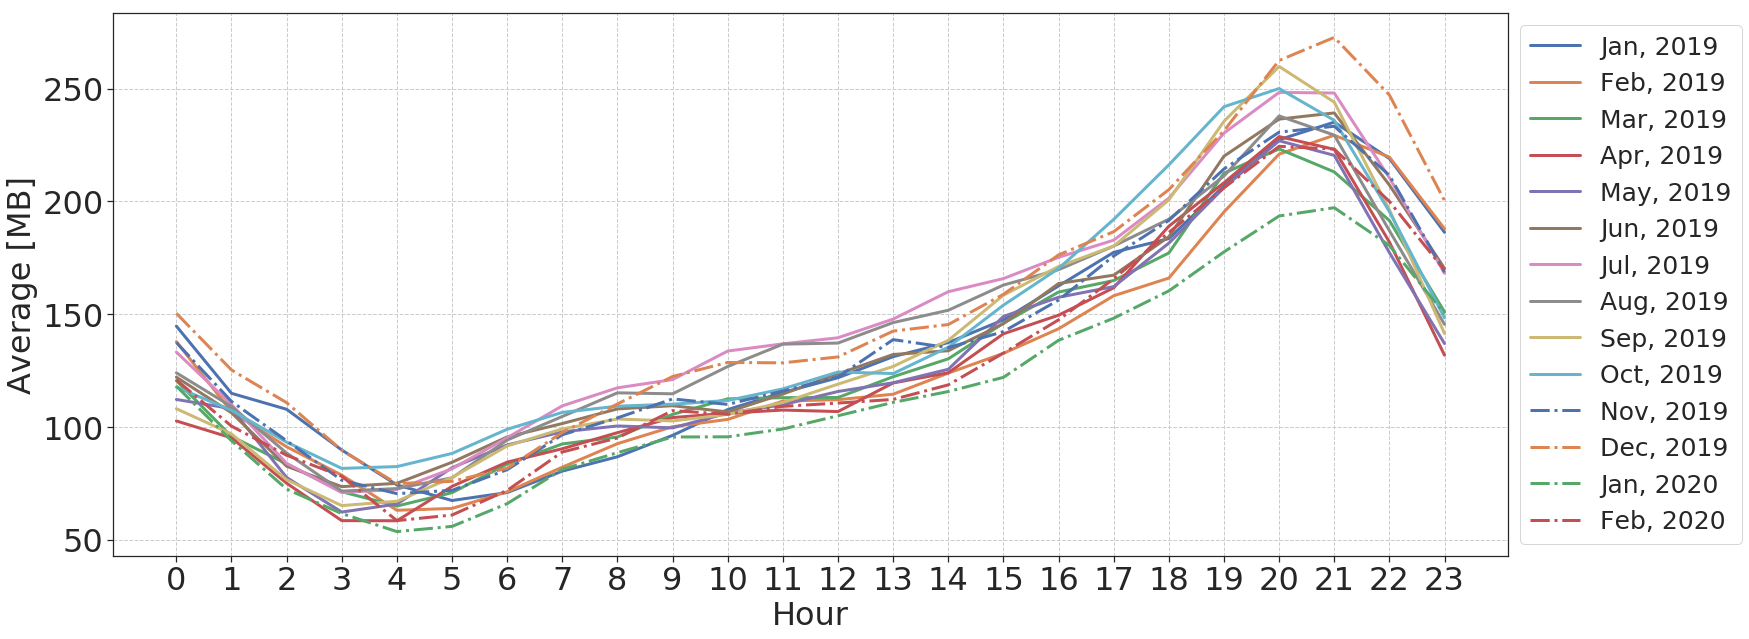
\includegraphics[width=0.49\linewidth]{figs/wenjun/download_wdays_before.png}%
    }
    \hspace*{\fill}
    \subfloat[\textbf{Pre-lockdown weekends.} Average volume of downloaded data per test unit, broken down by the hour of the day, on weekends in the pre-lockdown time period. \label{download-b}]{%
        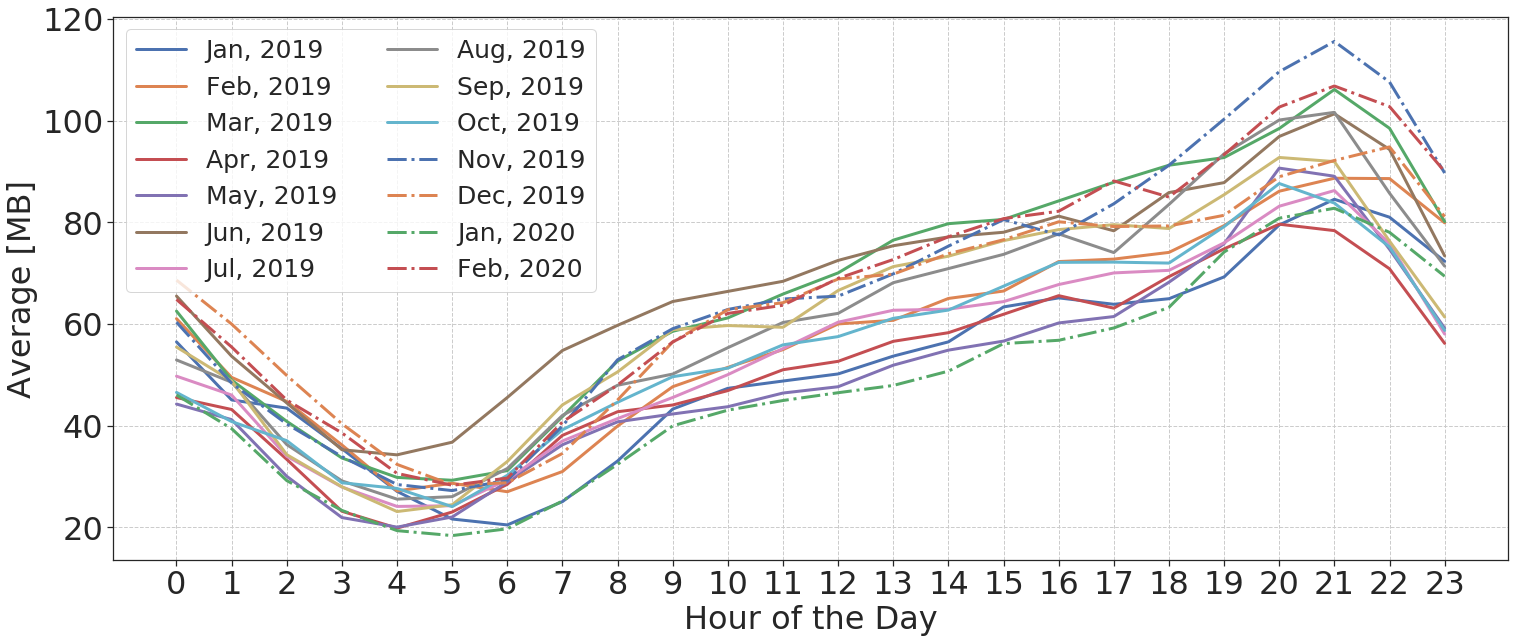
\includegraphics[width=0.49\linewidth]{figs/wenjun/download_wends_before.png}%
    }
    \\
    \subfloat[\textbf{Lockdown weekdays.} Average volume of downloaded data per test unit, broken down by the hour of the day, on weekdays in the lockdown time period. \label{download-c}]{%
        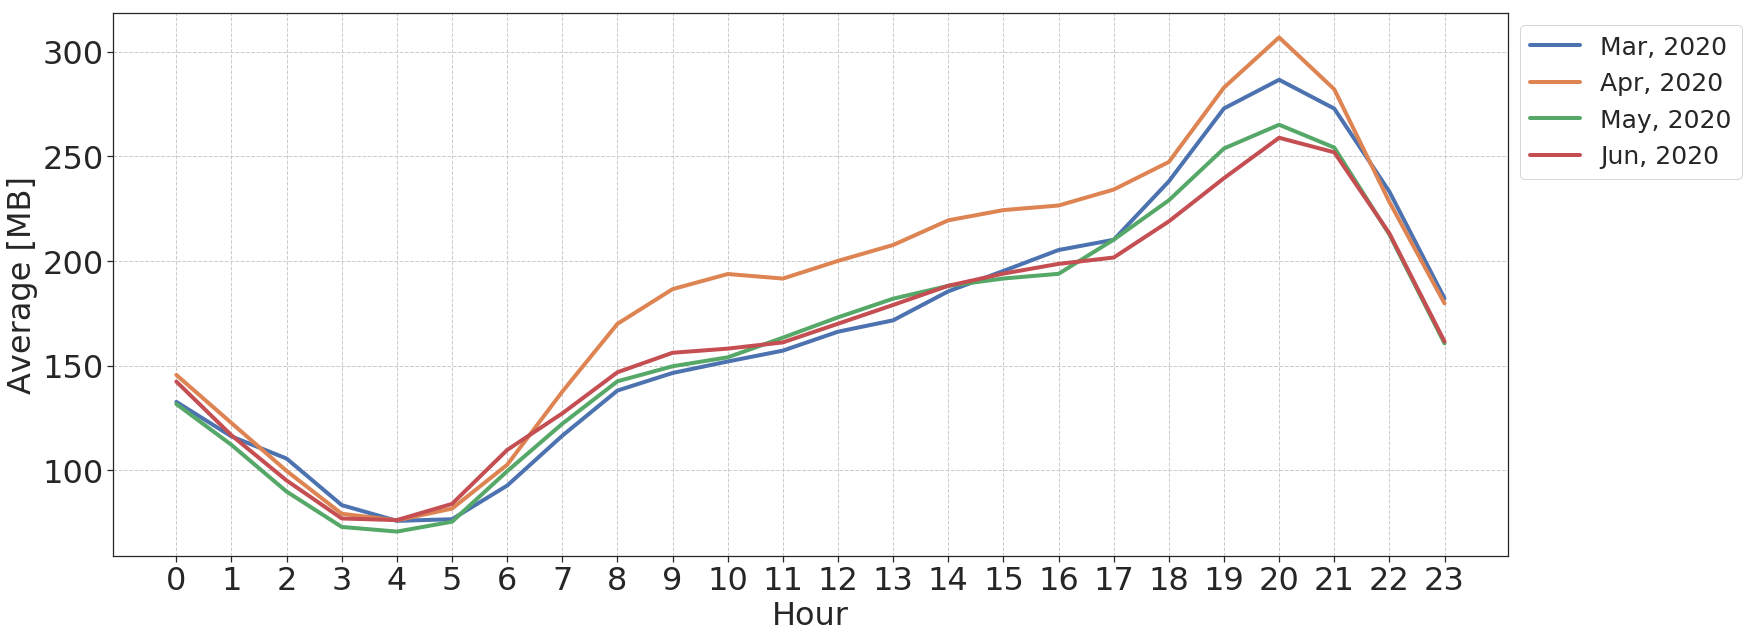
\includegraphics[width=0.49\linewidth]{figs/wenjun/download_wdays_after.png}%
    }
    \hspace*{\fill}
    \subfloat[\textbf{Lockdown weekends.} Average volume of downloaded data per test unit, broken down by the hour of the day, on weekends in the lockdown time period. \label{download-d}]{%
        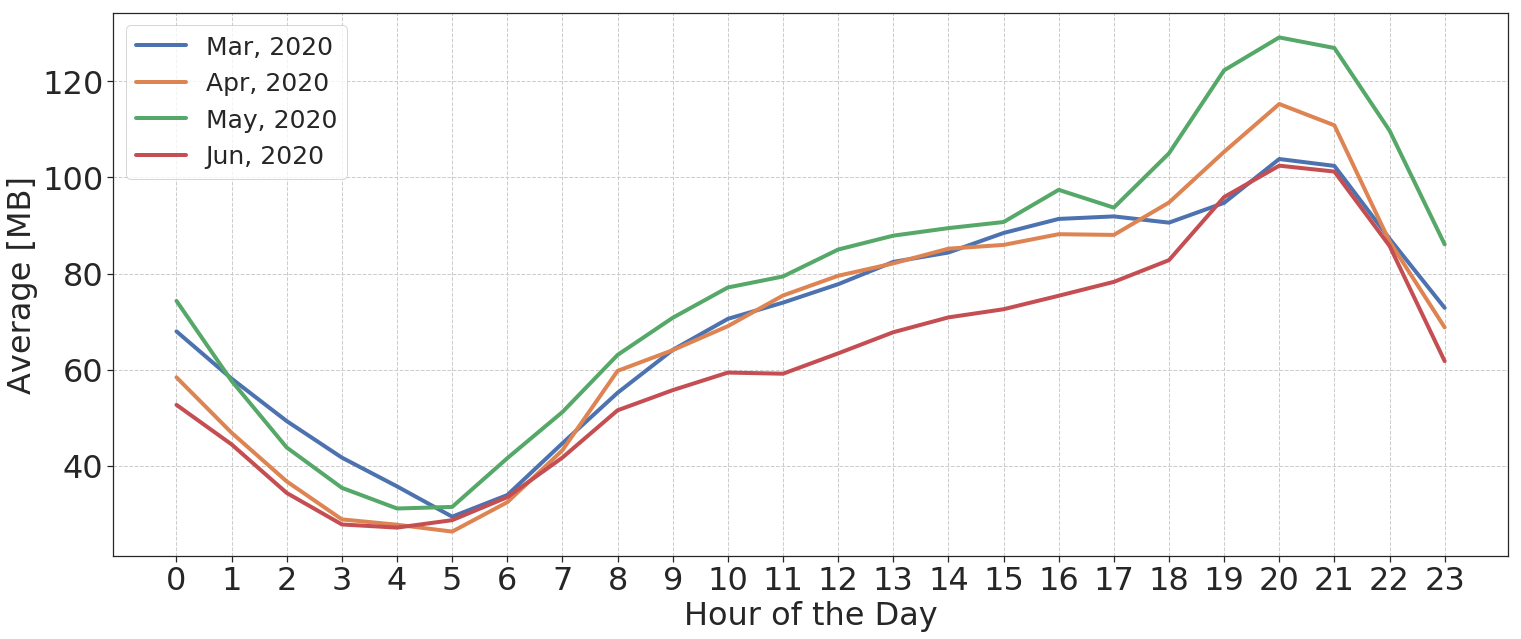
\includegraphics[width=0.49\linewidth]{figs/wenjun/download_wends_after.png}%
    }
    \\
    \subfloat[\textbf{2019 vs 2020 weekdays.} Average volume of downloaded data per test unit on weekdays in March-June compared between 2019 and 2020.
    \label{download-e}]{%
        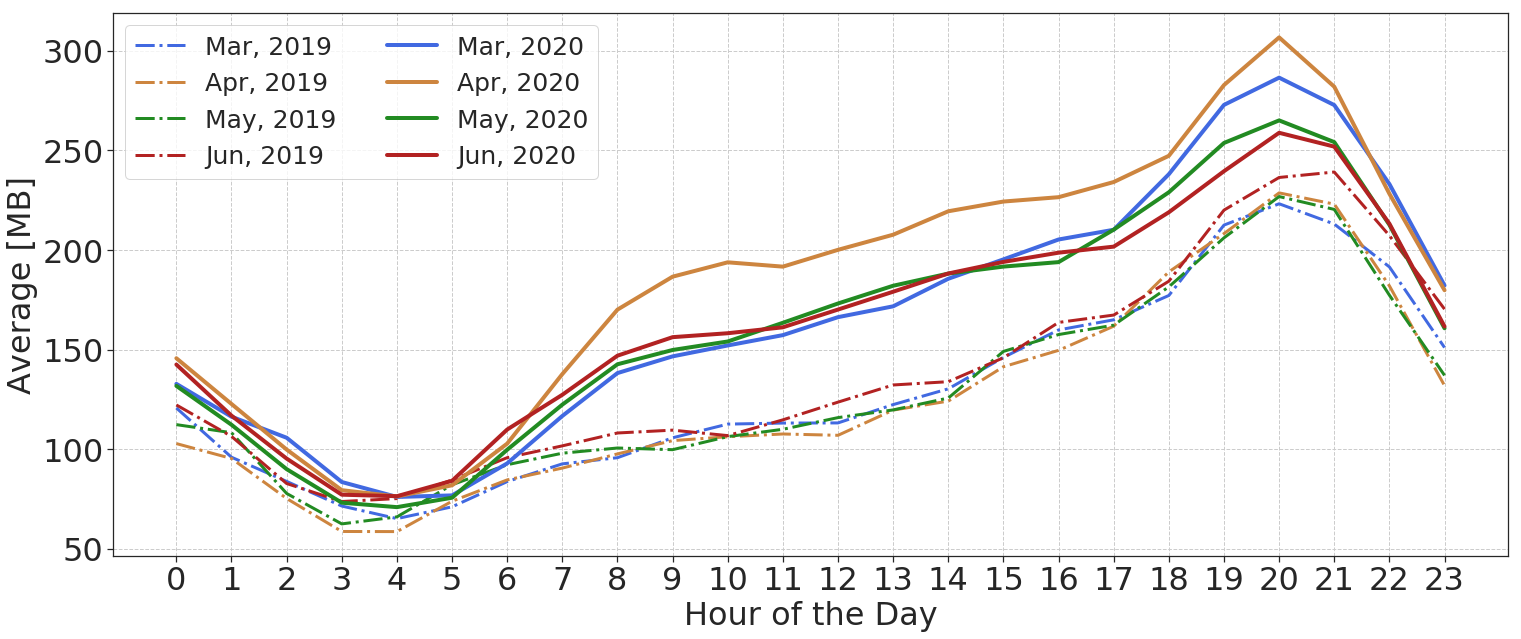
\includegraphics[width=0.49\linewidth]{figs/wenjun/download_wdays_compare_36.png}%
    }
    \hspace*{\fill}
    \subfloat[\textbf{2019 vs 2020 weekends.} Average volume of downloaded data per test unit on weekends in March-June compared between 2019 and 2020.
    \label{download-f}]{%
        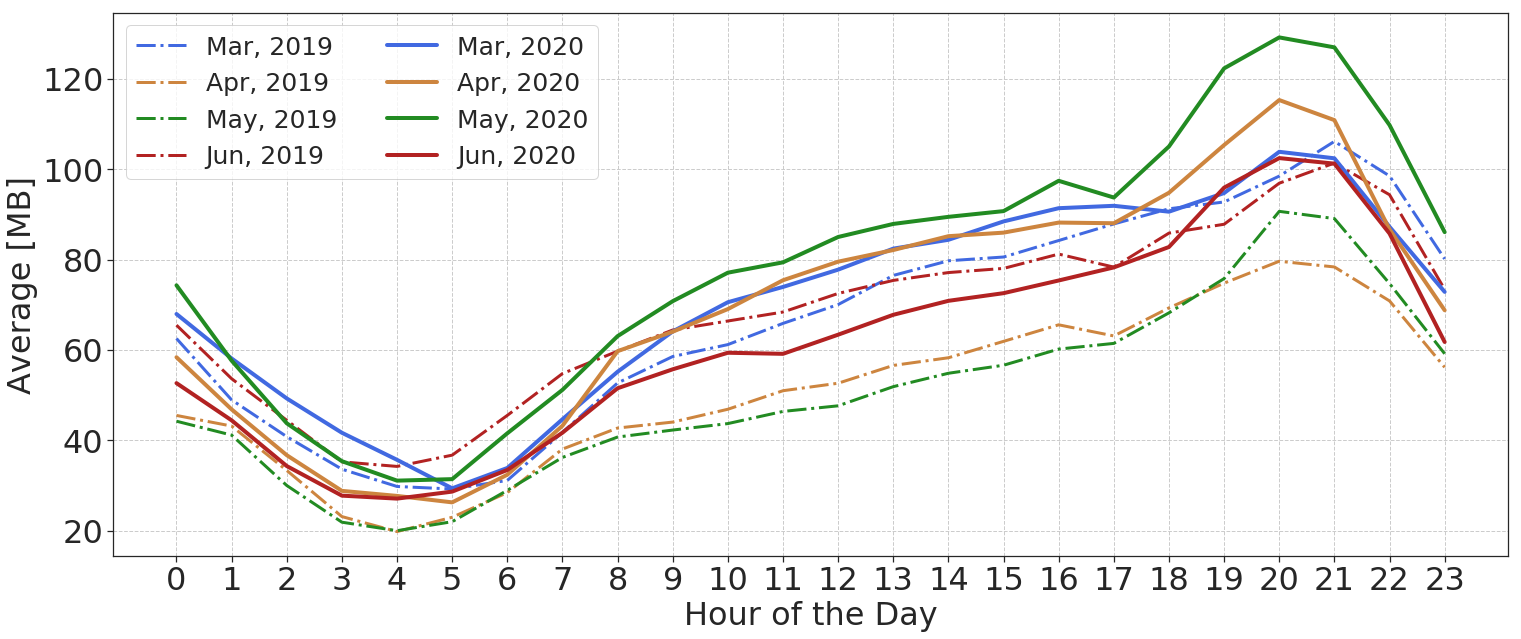
\includegraphics[width=0.49\linewidth]{figs/wenjun/download_wends_compare_36.png}%
    }

    \caption{Graphs comparing and contrasting the average hourly downloaded volume of data per test unit in various time periods. The peak is always between 18:00 and 22:00, which is the internet rush hour. The volumes in the lockdown time period are generally larger than the volumes in the pre-lockdown time period. Lockdown weekday traffic patterns start to resemble weekend patterns.}
    \label{fig:download-data-per-user-hours-fig}
\end{figure*}

\begin{figure*}[th]
    \centering
    \subfloat[\textbf{Pre-lockdown weekdays.} Average volume of uploaded data per test unit, broken down by the hour of the day, on weekdays in the pre-lockdown time period.
    \label{upload-a}]{%
        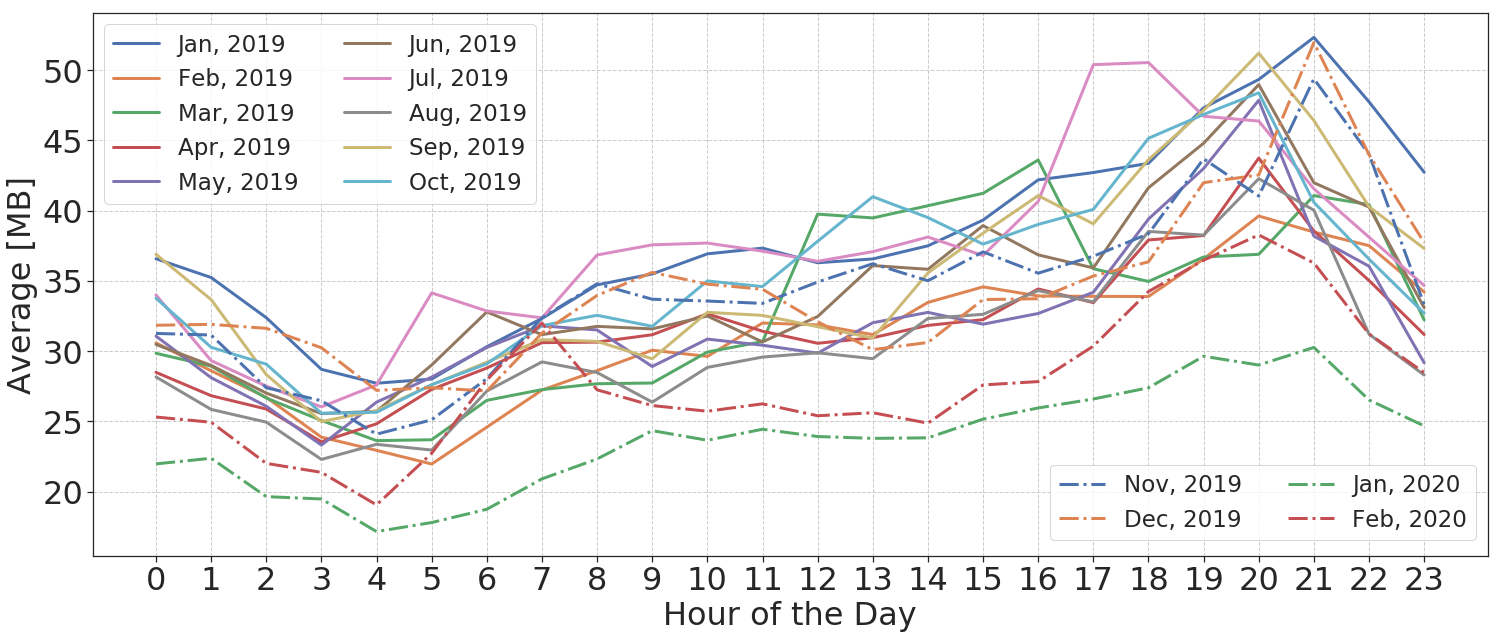
\includegraphics[width=0.49\linewidth]{figs/wenjun/upload_wdays_before.png}%
    }
    \hspace*{\fill}
    \subfloat[\textbf{Pre-lockdown weekends.} Average volume of uploaded data per test unit, broken down by the hour of the day, on weekends in the pre-lockdown time period.
    \label{upload-b}]{%
        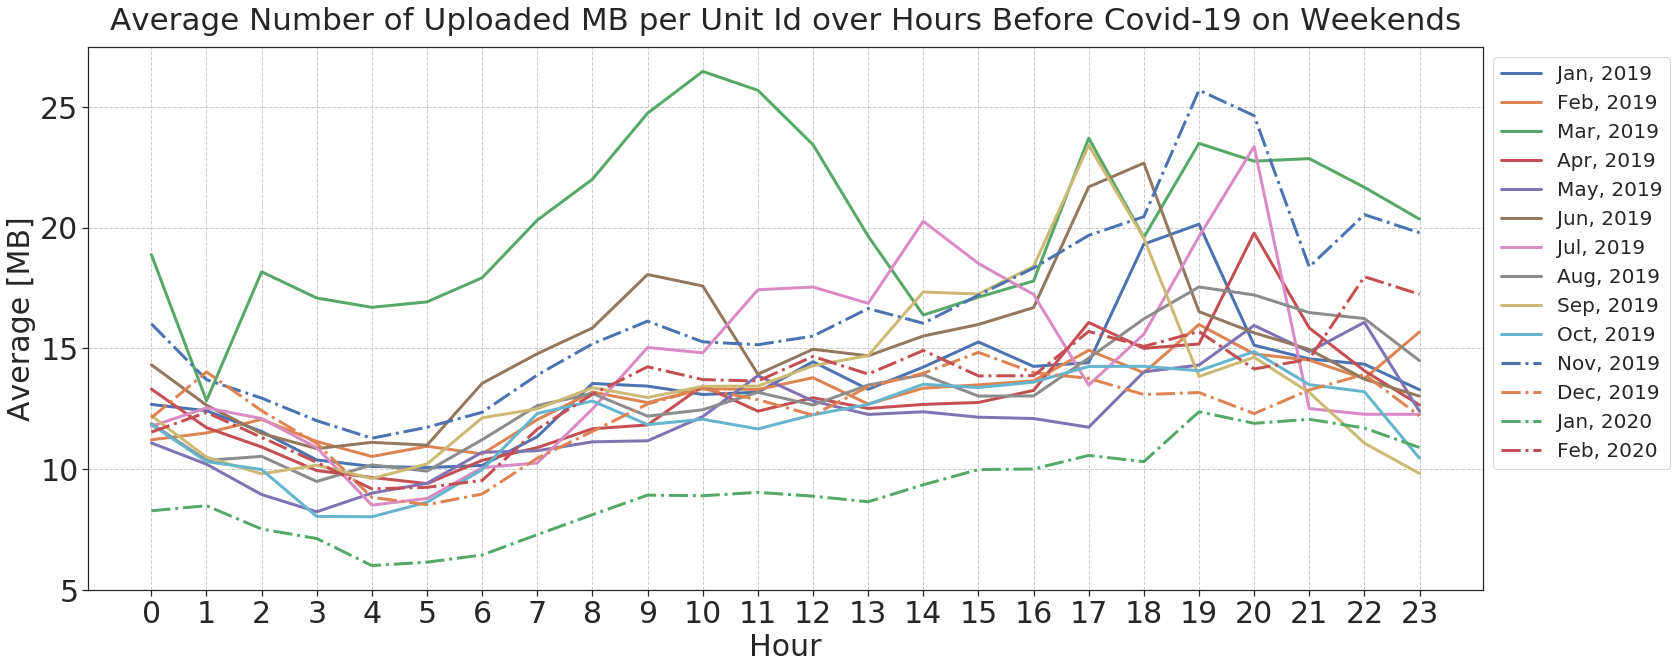
\includegraphics[width=0.49\linewidth]{figs/wenjun/upload_wends_before.png}%
    }
    \\
    \subfloat[\textbf{Lockdown weekdays.} Average volume of uploaded data per test unit, broken down by the hour of the day, on weekdays in the lockdown time period.
    \label{upload-c}]{%
        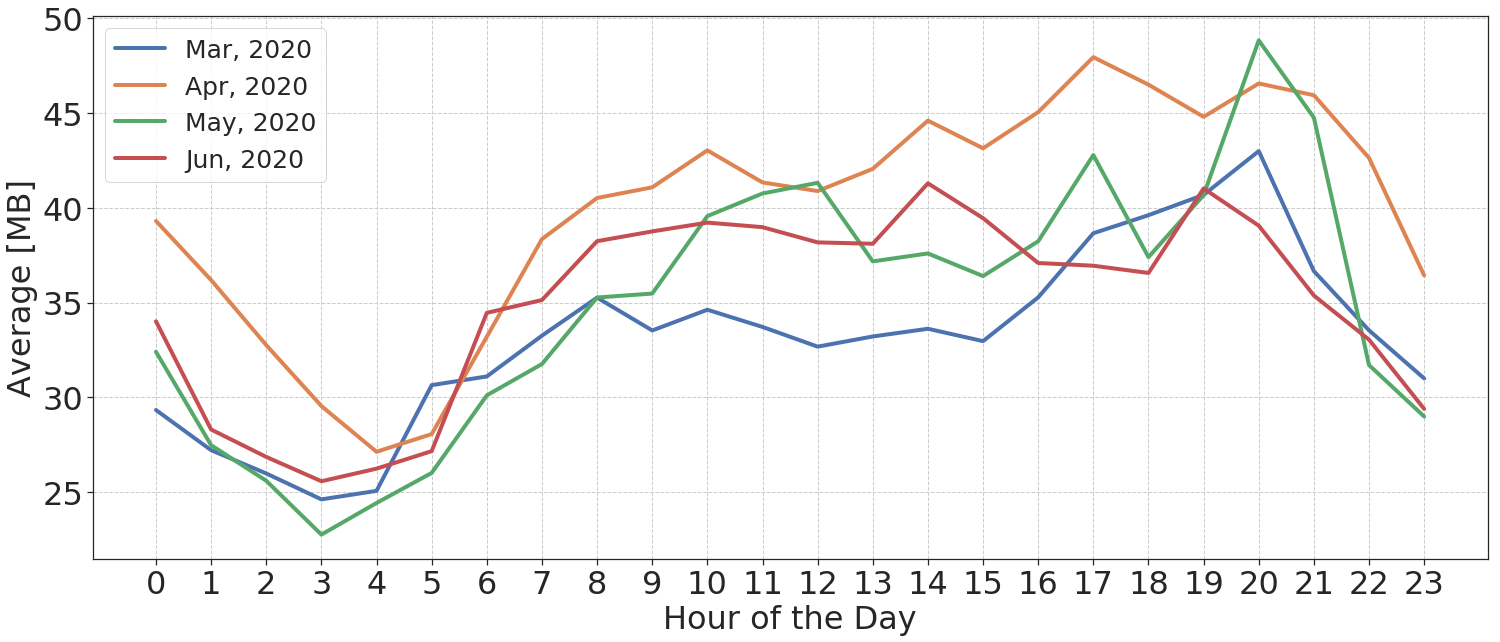
\includegraphics[width=0.49\linewidth]{figs/wenjun/upload_wdays_after.png}%
    }
    \hspace*{\fill}
    \subfloat[\textbf{Lockdown weekends.} Average volume of uploaded data per test unit, broken down by the hour of the day, on weekends in the lockdown time period. \label{upload-d}]{%
        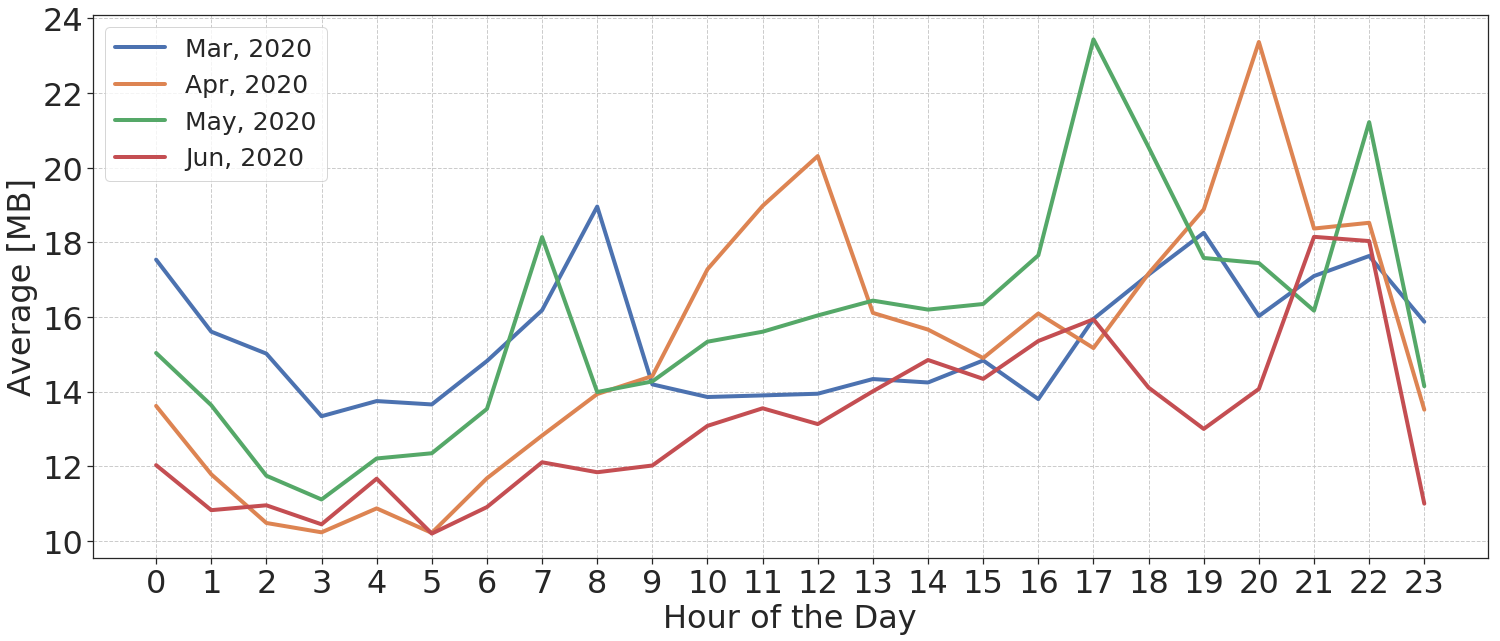
\includegraphics[width=0.49\linewidth]{figs/wenjun/upload_wends_after.png}%
    }
    \\
    \subfloat[\textbf{2019 vs 2020 weekdays.} Average volume of uploaded data per test unit on weekdays in March-June compared between 2019 and 2020.
    \label{upload-e}]{%
        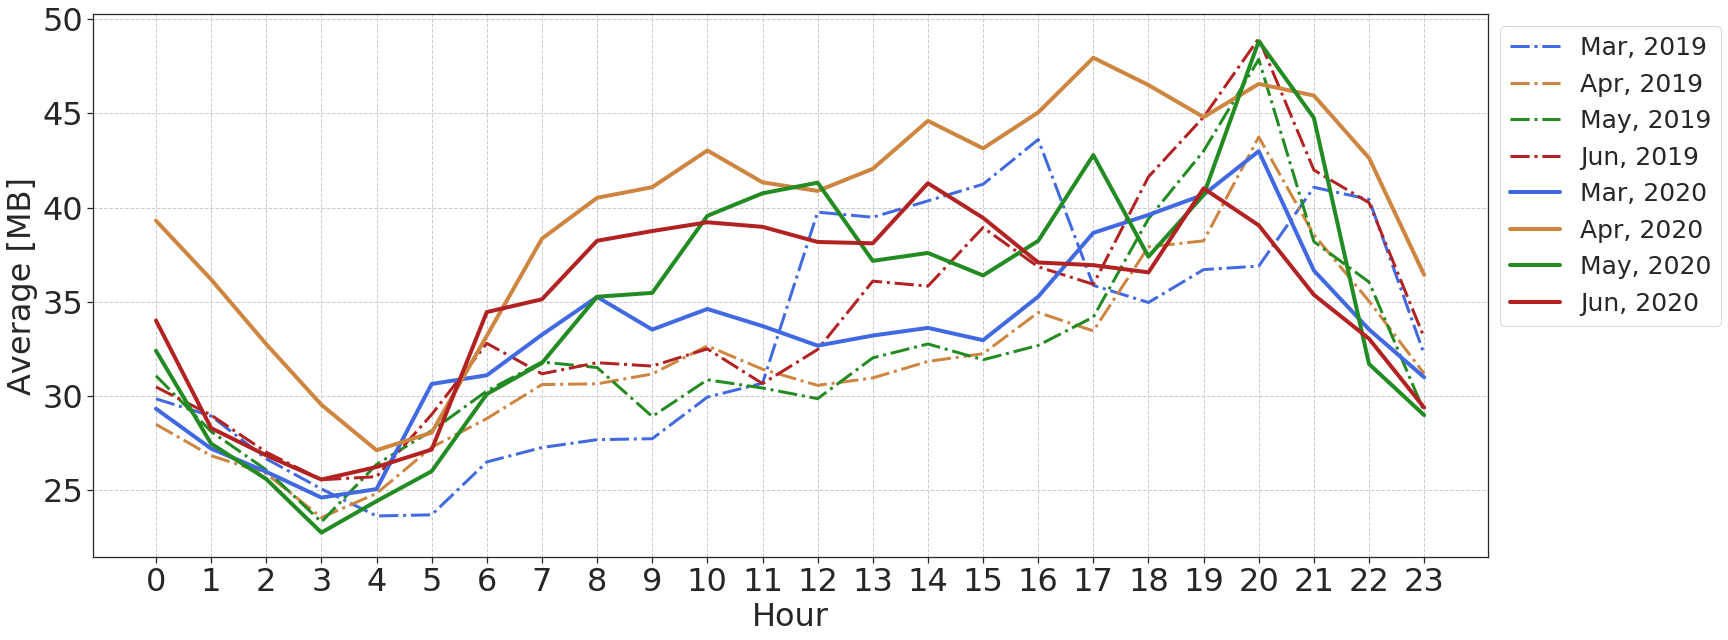
\includegraphics[width=0.49\linewidth]{figs/wenjun/upload_wdays_compare_36.png}%
    }
    \hspace*{\fill}
    \subfloat[\textbf{2019 vs 2020 weekends.} Average volume of uploaded data per test unit on weekends in March-June compared between 2019 and 2020.
    \label{upload-f}]{%
        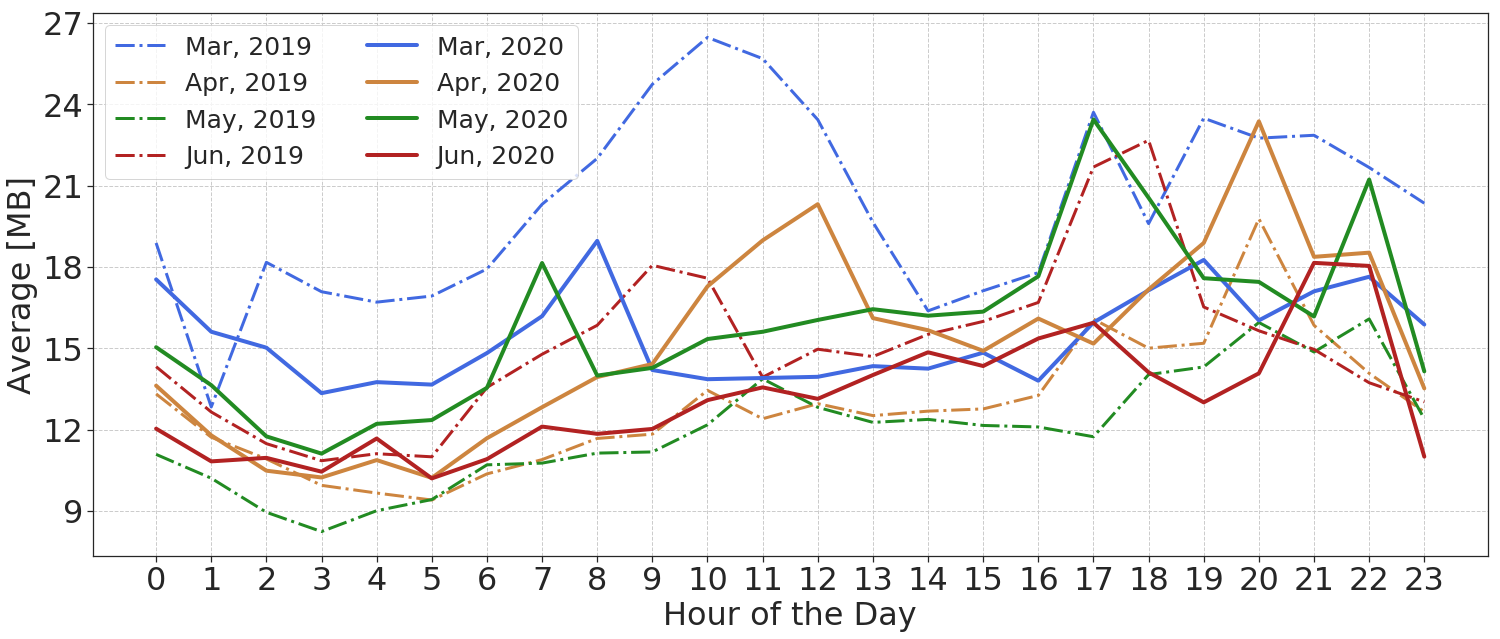
\includegraphics[width=0.49\linewidth]{figs/wenjun/upload_wends_compare_36.png}%
    }

    \caption{Graphs comparing and contrasting the average hourly upload volume of data per test unit in various time periods. Compared with download patterns, the lines in these graphs fluctuate more, especially on weekends. When comparing April and May between 2019 and 2020, we see an overall increase in uploaded data in 2020.}
  \label{fig:upload_data_per_user_hours_fig}
\end{figure*}


\section{Hourly Data Usage Patterns}\label{sec:hourly-data-usage-patterns}

Hourly data usage patterns (upload and download) could potentially provide insights into the behavior of fixed broadband internet users before and during the pandemic. Some applications such as music and video streaming generally increase the volume of downloaded data. Other applications such as \gls{VoIP}, video conferencing, or networked games influence the volume of uploaded data.

In this section, we study the average hourly data usage per test unit from multiple perspectives and attempt to correlate the observations with changing user behavior patterns during the lockdown. We contrast weekday and weekend patterns, analyze the differences in uploaded and downloaded traffic volumes, and compare with the data from the corresponding period of 2019 to eliminate potential seasonal differences.

The analysis in this section is primarily based on the ``datausage'' table from the \gls{FCC} \gls{MBA} raw dataset. That table keeps track of the total number of bytes received and transmitted by all user's devices within each hour of the day. For hourly analysis, we needed to translate \gls{UTC} timestamps to the test unit's local time using the unit profile dataset, as described in \cref{sec:methodology}. All graphs in this section were generated with measurements from approximately 3000 test units.

\subsection{Analysis of Download Patterns}\label{sec:analysis-of-download-patterns}

% internet rush hour explanation
All graphs in \cref{fig:download-data-per-user-hours-fig} show a traffic peak between 18:00 and 22:00 hours, also known as the internet rush hour~\cite{internetrushhour}. Most likely explanation for this peak is post-workday internet multi-media consumption for entertainment purposes, e.g., Netflix or Youtube.

% pre-lockdown weekday versus weekend
Graphs in \cref{download-a} and \cref{download-b} compare average weekday and weekend download traffic volumes in the pre-lockdown period, i.e., until end of February 2020. We clearly see that the overall average download volume is higher on weekdays. However, the distribution of activity throughout the day is different for weekdays and weekends. Between approximately 9:00 and 17:00, the weekend graph shows a relative increase in traffic volumes compared to the weekday graph and more variability month-to-month. This corresponds with the intuition that users typically use fixed broadband internet more during weekends when they are at home. The increase in variability can probably be partially explained by seasonal effects.

% pre-lockdown weekend versus lockdown weekend
\cref{download-b} and \cref{download-d} compare weekend traffic before and during lockdown. We see that the minimum and maximum weekend daily traffic levels are roughly the same before and during lockdown. In March--May 2020 we see a significant increase in daytime weekend traffic volumes (green, yellow, blue in \cref{download-d}) relative to the period before lockdown. Interestingly, daytime volumes return to their normal pre-lockdown levels in June 2020. This can be partially explained by the fact that many restrictions in effect since April were being relaxed by June. As a result, some users may have returned to spending their weekends outside of the home. % Maybe mention that this is consistent with "new normal" in one of the papers in Related Work.

% lockdown weekday versus weekend
When we compare lockdown weekdays with weekends in \cref{download-c} and \cref{download-d}, we see that the hourly weekday pattern starts to resemble weekend patterns. This trend is particularly visible for April 2020 (yellow). This trend is also clearly visible in \cref{download-e} which contrasts lockdown weekday data with weekday data from the same period of 2019. We clearly see that 2019 and 2020 curves cluster in two separate regions during daytime from roughly 8:00 to 18:00 hours. In other words, lockdown weekday download patterns morphed into weekend patterns. The same trend was observed by other authors in data from different vantage points.% Cite a specific paper.

% lockdown weekday detail
It is worth nothing that in \cref{download-c} April 2020 appears to be an outlier. All other lockdown months appear to converge to similar traffic levels. Somewhat lower traffic levels in May and June 2020 can be probably partially explained by: a) a new normal, b) relaxed lockdown restrictions. The traffic levels are highest in April because it is the first month in which most of the \gls{US} states were under a mandatory lockdown. Thus, this month represents the initial lockdown period during which a significant proportion of users was getting accustomed to working from home or online learning activities. The increase in evening traffic levels is likely due to social distancing restrictions \cite{lockdownsguide}, where people moved social activities to the internet.

% lockdown weekend detail
On weekends (\cref{download-f}), we see a small traffic increase in March, and the increases in April and May are substantial. Weekend June 2020 daytime traffic levels saw a relative decrease compared with June 2019 levels, except for the evening spike. One way to explain the difference might be that after months of restrictions people try to spend weekends more outside their homes. This pattern coincides with the policies related to COVID-19 in the \gls{US}: the height of restriction was at the end of March and the beginning of April, and some restrictions were being relaxed in the mid-late May or June in many states~\cite{covid19restriction}.

We conclude that people use fixed broadband internet more and download more data because of COVID-19 and its related policies (e.g., lockdown, quarantine, work from home, etc.).

\subsection{Analysis of Upload Patterns}\label{sec:analysis-of-upload-patterns}

\cref{fig:upload_data_per_user_hours_fig} shows several plots of hourly average uploaded data. As expected, there is significantly more noise and fluctuation in these plots (particularly weekends), compared with the download plots in \cref{fig:download-data-per-user-hours-fig}.

We note that we have no explanation for the morning spike in March 2019 shown in \cref{upload-b}. Unlike the corresponding download patterns, hourly upload patterns before lockdown show little difference between weekdays and weekends, partly due to the noise.

 The average uploaded data levels April and May 2020 are larger than those in 2019, but in March and June, that is not the case (\cref{upload-e} and \cref{upload-f}). Possible reasons might be similar to those discussed earlier: the majority of \gls{US} states enforced peak lockdown restrictions at the end of March and the beginning of April. Some of the restrictions ended in mid-late May or June in some states~\cite{covid19restriction}.

 On weekdays, the daytime average uploaded data levels in April, May, and June 2020 are much larger than those in the corresponding months of 2019. On weekends, the increase is relatively smaller than on weekdays.

\subsection{The Data Consumption}
\label{sec:the-data-consumption}
In this sub-section, we present the results that show how COVID-19 changed the amount of average data downloaded and uploaded per user.

\subsubsection{Data Downloaded}
\label{sec:download-data-consumption}

In order to analyze the impact of COVID-19 on the amount of data downloaded, we calculated the average value of data downloaded per user each month in the timeline of January-March 2020. After the averages were computed, Figure \ref{fig:download2020} was generated and it shows how it has changed from January to March.

\begin{figure}
\centering
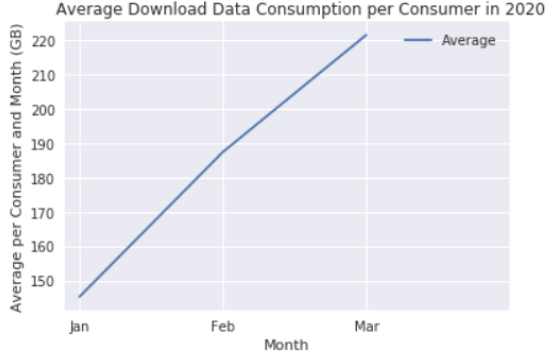
\includegraphics[width=1.0\linewidth]{figs/download2020.PNG}
\caption{Graph showing the average consumption of downloaded data per user for the first three months of 2020.}
\label{fig:download2020}
\end{figure}

As Figure \ref{fig:download2020} shows, in January the average amount of data downloaded per consumer was approximately \SI{145}{\giga\byte}, and in March this value went up to approximately \SI{221}{\giga\byte}. This represents an increase of approximately 53\% in the average alue of data downloaded per consumer. As Figure \ref{fig:downloadup2019} shows, in 2019, from January to March there was actually a decrease in the value of data downloaded (average for download is represented by the red line). Thus, one could conclude that the trend in data downloaded per user changed from 2019 to 2020, since instead of decreasing, the average per consumer increased considerably from January to March in 2020. Therefore, considering that the COVID-19 outbreak is the most extenuate different circumstance if we compare these two periods, it is possible to conclude that this new trend in the quantity of data downloaded was a consequence of the pandemic, since it cause stay-at-home and lockdown orders around the U.S. in the first semester of 2020. Hence, as people stayed at home more in March 2020, one possible explanation for this change in the value of downloaded data could be that they spent more time on online entertainment, e.g., video streaming services and games as well as joined online classes and working meetings regularly, which made the their average amount of data downloaded to go up and shows that people tended to comply with stay at home orders.

\begin{figure}
\centering
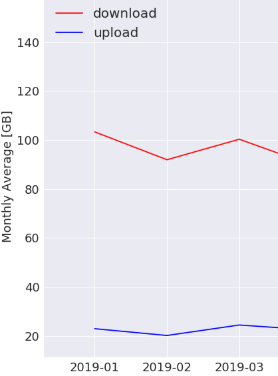
\includegraphics[width=0.5\linewidth]{figs/downloadup2019.PNG}
\caption{Graph showing the average consumption of downloaded and uploaded data per user for the first three months of 2019.}
\label{fig:downloadup2019}
\end{figure}

\subsubsection{Uploaded Data}
\label{sec:upload-data-consumption}

Similarly to the average downloaded data analysis, while computing the average amount of data uploaded per consumer for the period of January-March of 2020, we could observe an increase. Figure \ref{fig:upload2020} shows that in January, the average value of data uploaded per consumer was approximately \SI{25}{\giga\byte} while in March it increased to approximately \SI{37}{\giga\byte}. These numbers show that there was an increase in the value of approximately 38\%. Moreover, Figure \ref{fig:downloadup2019} also shows the average of uploaded data per consumer in 2019. According to the graph (average for upload is represented by the blue line), in 2019 there was a small increase from January to March. However, this increase was less than 2\%, which showing an increase not as significant as the increase observed between the same period in 2020. Hence, it is possible to conclude that there was also a shift in the trend of the average data uploaded per consumer from January to March comparing 2019 and 2020. Therefore, while looking for an explanation to this rise in data uploaded per consumer, we should consider the fact that classes went online and that many companies started remote work in the middle of March due to the pandemic. Online meetings operated by Zoom, Webex and Microsoft Teams became part of the routine of many Americans, which affected not only the average value of data downloaded per user, but also and more importantly, the average amount of data uploaded per user. This once again confirms that COVID-19 impacted the usage of internet and changed the amounts of data downloaded and uploaded, creating new trends and behaviors. 

\begin{figure}
\centering
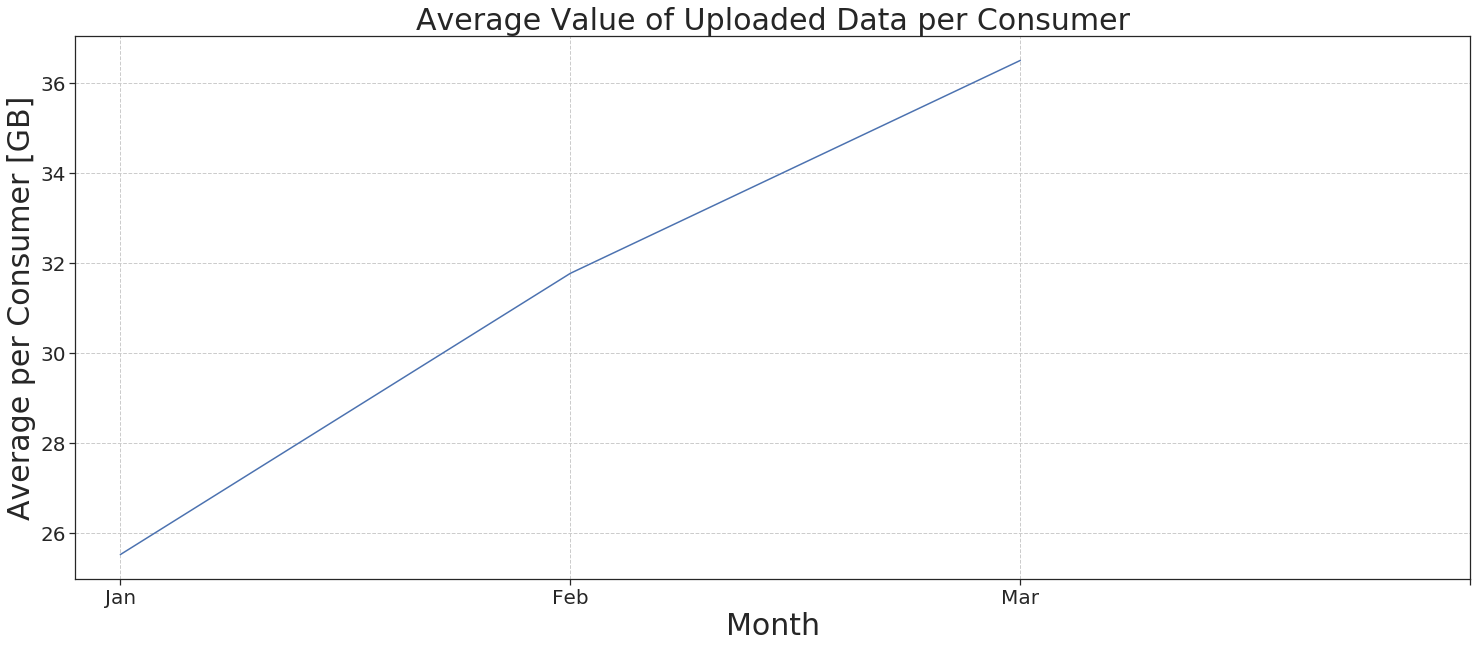
\includegraphics[width=1.0\linewidth]{figs/upload2020.PNG}
\caption{Graph showing the average consumption of uploaded data per user for the first three months of 2020.}
\label{fig:upload2020}
\end{figure}

Therefore, it can be concluded that the COVID-19 changed internet usage in the US in the first quarter of 2020. The increase in the averages of data downloaded and uploaded per consumer from January to March in 2020 explicitly shows that there was an outside event that impacted the usage of internet, making it higher than it would be expected based on the trends of internet usage established in the same period of 2019. Since there was not any other major event influencing internet usage in March 2020, it is possible to conclude that this increase in the average amount of data downloaded and uploaded happened due to COVID-19, since people were using internet more while they were complying to stay-at-home orders and quarantining.

\subsection{Average Speed}
\label{sec:average-speed}
Besides analyzing the average amount of data downloaded and uploaded per consumer in 2020, we also analyzed how the average speed experienced by consumers changed from January to March 2020. By knowing that the average value of data used per user increased significantly, it could be expected a change in the average speed that people experienced in the middle of quarantine, considering the expressive increase in data used.

\subsubsection{Average Download Speed}
\label{sec:average-download-speed}

In order to understand how the COVID-19 outbreak impacted the average download speed experienced by consumers, we calculated the ratio between the average download speed that users experienced between January and March 2020. Defining $S_{\text{download}}$ as the download speed, the ratio was computed by the following formula:

\begin{equation}
AVG_{S_{\text{download}}}\% = \frac{AVG_{S_{\text{download}},\, \text{Mar}}-AVG_{S_{\text{download}},\, \text{Jan}}}{AVG_{S_{\text{download}},\, \text{Jan}}}\times 100
\end{equation}

% \begin{equation}
% ratio= ((av.speed.Mar - av.speed.Jan)/ av.speed.Jan)*100
% \end{equation}

Figure \ref{fig:downloadspeed2020} shows the results of the compilation of the ratios in a CDF and according to this graph, it is possible to infer that approximately 60\% of the users experienced a decrease in their average download speed from January to March. However, the decrease was not too significant, since for most part of the users, it was smaller than 5\%. Thus, while a significant number of users experience a decrease in average download speed as other studies suggest, not many experience a severe decrease. In the article \textit{Internet Speed Analysis: Top 200 Cities, March 15th – 21st} \cite{cooper}, Cooper affirms that although some ISPs were able to hold up the increase in  internet consumption, some cities felt the impact of the increase in data consumption leading users to experience a decrease in their download speed, e.g., the download speed in New York City decreased by 24\% in March. This expressive decrease in the download speed in some cities is a result of the decrease of average download speed that consumers have experienced from January to March in 2020 and vice-versa.

\begin{figure}
\centering
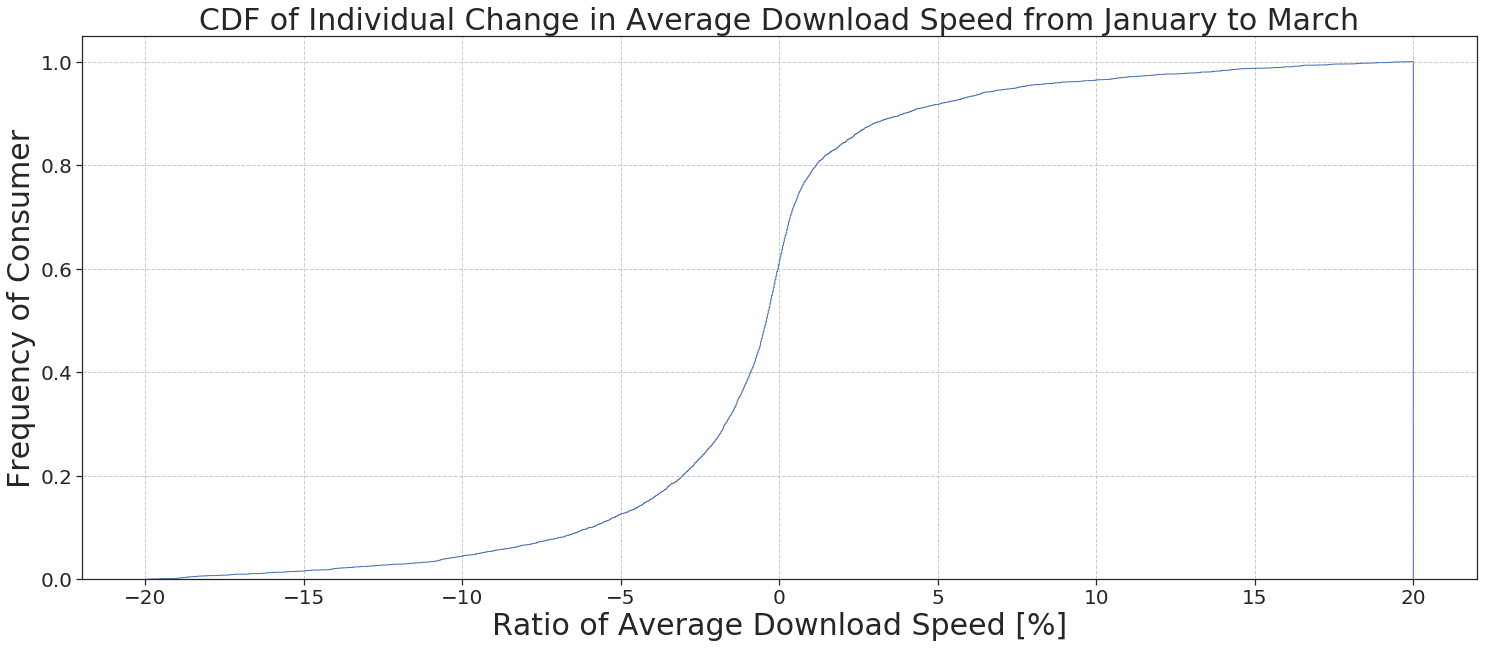
\includegraphics[width=1.0\linewidth]{figs/downspeed.PNG}
\caption{CDF that shows the ratios of average download speed experienced per consumer between January and March of 2020.}
\label{fig:downloadspeed2020}
\end{figure}

\subsubsection{Average Upload Speed}
\label{sec:average-upload-speed}
Similarly to the average download speed, we also computed the ratio between the average upload speed experienced by users between January and March 2020. Defining $S_{\text{upload}}$ as the upload speed, similar to the ratios for average download speed, the formula used can be represented as:

\begin{equation}
AVG_{S_{\text{upload}}}\% = \frac{AVG_{S_{\text{upload}},\, \text{Mar}}-AVG_{S_{\text{upload}},\, \text{Jan}}}{AVG_{S_{\text{upload}},\, \text{Jan}}}\times 100
\end{equation}

% \begin{equation}
% ratio= ((av.speed.Mar - av.speed.Jan)/ av.speed.Jan)*100
% \end{equation}

Figure \ref{fig:uploadspeed2020} shows the compiled result of these ratios and, according to this graph, approximately 70\% of consumers (called unit-ids in the graph) saw their average upload speed decreasing from January to March 2020. As people transitioned most of their activities to a virtual environment, such as working and studying from home and had to log in calls and virtual conferences more often, it could be expected an increase in data upload (as Figure \ref{fig:upload2020} shows) and, consequently, a decrease in the average upload speed, since there were more data being uploaded than before. Again, similarly to the situation observed with the download speed, while 70\% of consumers experienced a decrease in their upload speed, this decrease was also modest, mostly less of 5\%.

\begin{figure}
\centering
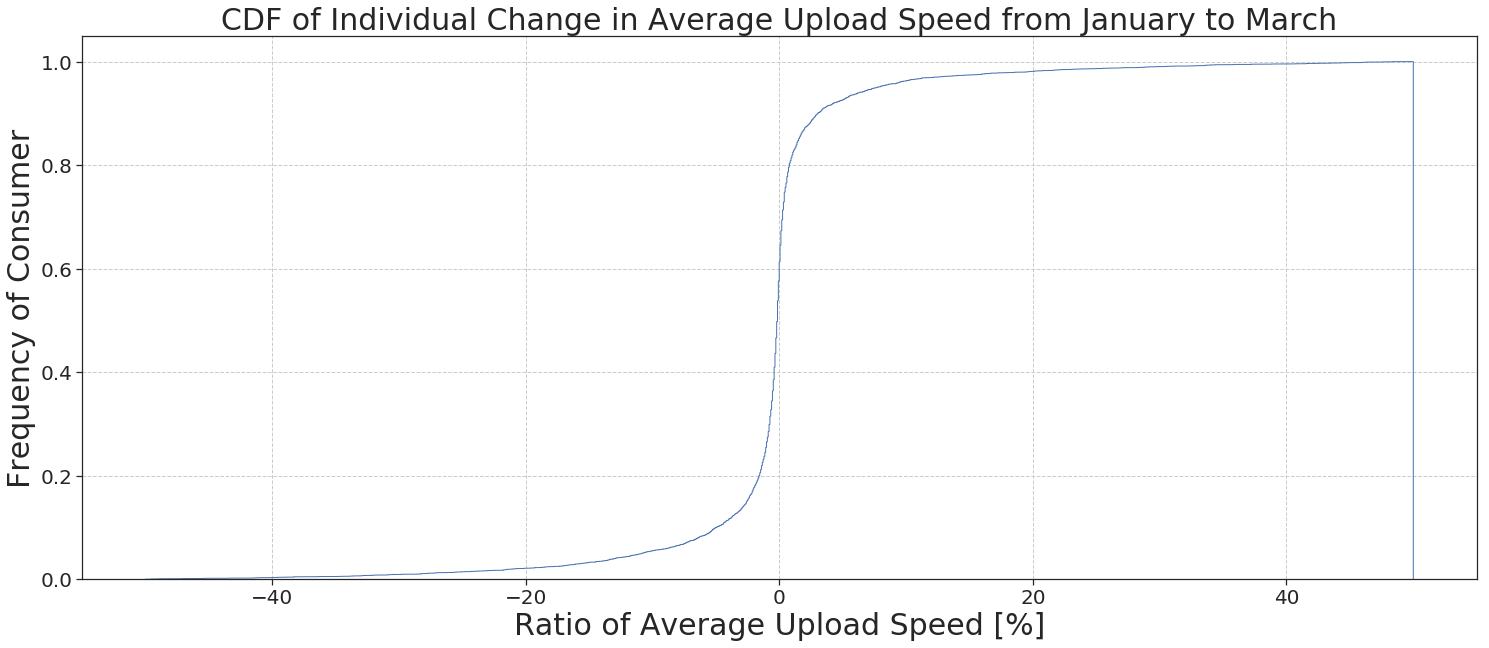
\includegraphics[width=1.0\linewidth]{figs/uploadspeed.PNG}
\caption{CDF that shows the ratios of average upload speed experienced per consumer between January and March of 2020.}
\label{fig:uploadspeed2020}
\end{figure}

\subsection{Consumers with the heaviest internet consumption}
\label{sec:analyzing-the-users-with-the-highest-internet-usage}

One component analyzed in this research was how the users who extensively used internet before the pandemic, have been using it after the COVID-19 outbreak. This analyzes hopes to gain more behavioral insights about people's internet consumption. Thus, we identified the 10\% of users (approximately 500 users) who had the highest averages of data downloaded and uploaded in January 2020 and computed the ratio of average usage between January and March in order to find out if their usage increased or decreased after COVID-19 hit the country in early March.

\subsubsection{Heavy Download Users}
\label{sec:heavy-download-users}

In order to analyze the data usage of only heavy users, we computed the ratio of data downloaded between January and March for users who downloaded more than \SI{400}{\giga\byte} in January, in order words: we computed the ratios of data downloaded for approximately 10\% of the users who downloaded the most data in January. We applied the following formula to calculate the ratios:

\begin{equation}
\frac{Data_{\text{downloaded},\, \text{March}}}{Data_{\text{downloaded},\, \text{January}}}
\end{equation}

% \begin{equation}
% ratio= data.downloaded.Mar/ data.downloaded.Jan
% \end{equation}

After computing the ratios for the 10\% of users who downloaded the most data in January, we computed the CDF shown in Figure \ref{fig:heavydown}.

\begin{figure}
\centering
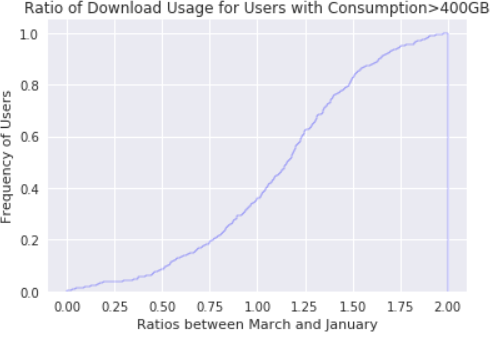
\includegraphics[width=1.0\linewidth]{figs/heavydown.PNG}
\caption{CDF that shows the ratios of average amount of data downloaded per consumer between January and March 2020 for consumers who downloaded more \SI{400}{\giga\byte} in January (top 10\% of consumers for data downloaded in January).}
\label{fig:heavydown}
\end{figure}

The graph shows that approximately 40\% of the users increased their consumption of data downloaded. While this number is surprising, considering that before quarantine and stay-at-home orders took place these users were already using internet on its maximum capacity, a possible explanation to an increase in internet used for these users is that during quarantine, they spent even more time using video streaming service, e.g., Netflix and YouTube. According to Kovacs \cite{kovacs}, the world suffered from a more extensive internet traffic in March which was primarily caused by video streaming services. Kovacs also explained in her paper \textit{U.S. broadband networks rise to the challenge of surging traffic during the pandemic} that 24\% of internet traffic in the U.S. was caused by video services and that as a response, in March Netflix reduces its streaming speed and YouTube only allowed standard definition on its videos worldwide.



\section{Challenges}
\label{sec:challenges}
Because we were working with a big data set, in total \SI{300}{\giga\byte} of data, one of the main challenges that we faced was to find an application that would be able to process all this data. By talking to my supervisors, we decided to use a virtual machine on Google Cloud because we thought it would be enough to treat and process all the data sets. However, even using Google Cloud, the virtual machine run out of memory and it was necessary find different ways to storage the data, such as transitioning to BigQuery. Moreover, even though this is a professional data set gathered by FCC, there was still some invalided and noisy data and some lack of data description, e.g., outdated information about Whiteboxes. These implications related to the data set also led to some additional challenges to analyze it.

\section{Conclusion}
\label{sec:conclusion}

The study of average download data and upload data usage per user over hours on each month indicates that the policies related to COVID-19, such as lockdown, stay-at-home, work-from-home, etc., do increase the usage of internet in the United States on both weekdays and weekends. 


Furthermore, based on the graphs and information presented, we found that the COVID-19 outbreak has impacted the consume of internet in the US. In terms of average consumption per user, from January 2020 to March 2020 (before and after COVID-19 hit the country) increased by 53\% for downloaded data and by 38\% for uploaded data. In addition to that, approximately 70\% of consumers experienced a decrease in their average download speed in March if compared to their average download speed in January, and approximately 80\% of users noticed a decrease in their average upload speed. These numbers show some of the impacts of COVID-19 in internet usage since this has been the most influential external factor to internet consumption in the US. Through these results that show that people indeed consumed more data in March, it can be inferred that people tended to comply to the stay at home orders and started doing most of their daily activities e.g., work and study, in a virtual environment.

\section{Future Work}
\label{sec:future-work}

As this project is a working in progress, some of the next steps would be continuing analyzing the changes in internet consumption, e.g., how consumption changed in business hours and changes related to different geographic regions in the US, and also analyzing changes in latency.

\section{Acknowledgements}
\label{sec:acknowledgements}

Jessica Moreira was funded by Craig Newmark Philanthropies while working on the project. She would also like to thank to the DIMACS REU summer 2020 research program and Barnard Computer Science department for additional support.

\bibliographystyle{IEEEtran}
\bibliography{bibs/references}
\end{document}
